O Banco de Baterias tem a função de armazenar a energia remanescente produzida pela turbina, com o intuito de manter todos os sensores e equipamentos da torre de controle, em caso de emergência, em perfeito funcionamento. Também será necessário uma bateria na turbina para manter o funcionamento dos sensores lá localizados.
O conjunto de baterias deve suprir toda a demanda da casa de máquinas. O consumo da casa de máquinas foi estimado em 36kW e dos sensores em torno de 1kW. Em caso de emergência, o Banco de Baterias deve manter o funcionamento da casa de máquinas por, aproximadamente, 2 horas.
 Para dimensionar o banco de baterias é necessário ter a potência dos equipamentos que serão alimentados pelas baterias, o tempo de funcionamento dos equipamentos e o uso do sistema. 
As baterias escolhidas foram as Baterias Estacionárias Moura Clean 220 Ah. As especificações estão em negrito no quadro a seguir:
\FloatBarrier
\begin{figure}[!ht]
\centering
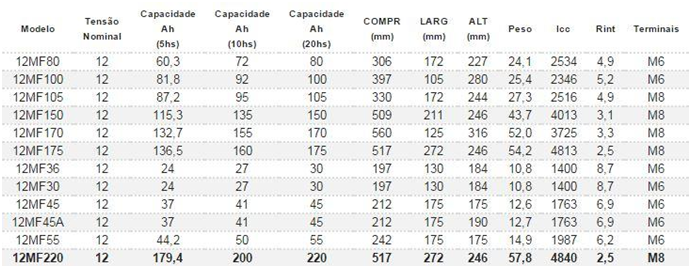
\includegraphics[scale=0.7]{editaveis/figuras/bateria}
\caption[Especificações das baterias]{Especificações das baterias\footnotemark}

\label{bateria}
\end{figure}
\footnotetext{Disponível em: https://www.energiapura.com/content/bateria-estacionária-moura-clean-220-ah}
\FloatBarrier

A potência e o tempo de funcionamento são utilizados para calcular o consumo. O consumo é calculado através da seguinte fórmula:
\FloatBarrier
\begin{figure}[!ht]
\centering
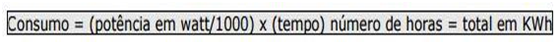
\includegraphics[scale=1]{editaveis/figuras/consumo}
\caption[Consumo]{Equação de consumo\footnotemark}
\label{consumo}
\end{figure}
\footnotetext{Disponível em: http://www.aneel.gov.br/arquivos/PDF/17-05\_materia1\_3.pdf}
\FloatBarrier

Substituindo os valores na fórmula, obtêm-se:
\FloatBarrier
\begin{figure}[!ht]
\centering
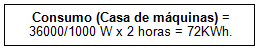
\includegraphics[scale=1]{editaveis/figuras/consumo_sub}
\caption[Consumo]{Cálculo do consumo da casa de máquinas}
\label{consumo}
\end{figure}
\FloatBarrier

Para mensurar a quantidade de baterias necessária, deve-se converter Kwh para Ah (ampère-hora). Para isso, utiliza-se a seguinte fórmula:
\FloatBarrier
\begin{figure}[!ht]
\centering
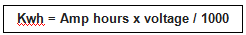
\includegraphics[scale=1]{editaveis/figuras/bateria_necessaria}
\caption[Equacao conversão]{Equação conversão Kwh para Ah\footnotemark}
\label{conversao}
\end{figure}
\footnotetext{Disponível em: http://www.hupsolar.com/questions-about-HUP-solar-batteries/How-to-convert-from-Kilowatt-hours-to-Amp-hours}
\FloatBarrier

Substituindo os valores na fórmula, obtêm-se:
\FloatBarrier
\begin{figure}[!ht]
\centering
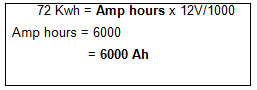
\includegraphics[scale=1]{editaveis/figuras/conversao_sub}
\caption[Conversao]{Cálculo da quantidade de baterias necessárias}
\label{conversao}
\end{figure}
\FloatBarrier

Analisando as especificações da bateria, observa-se a capacidade em Ah (5 horas) no valor de 179,4. Para o nosso projeto, considerando 2,5 horas, o valor é de aproximadamente 160 Ah. Isso significa que, para uma descarga de 2,5 horas serão consumidas 160 Ah.  

Para suprir a necessidade de manter a torre de controle ativa por duas horas, considerando que as baterias não possam ser descarregadas completamente e que tenha uma margem de segurança, deve-se utilizar várias baterias conectadas em série.
Dividindo a quantidade de ampères necessárias pela quantidade de ampères de uma bateria, é possível obter a quantidade de baterias necessárias para o projeto. O valor obtido é de 37 baterias.
Para manter os sensores que são acoplados na turbina em funcionamento em caso de emergência, a energia necessária é de aproximadamente 1 kW. Utilizando as fórmulas citadas acima; para manter o sistema de sensores por duas horas é necessário 2kWh.

Convertendo 2kWh, obtêm-se 166,66 Ah. Analisando a capacidade da bateria (aproximadamente 160 Ah (2,5 horas)), percebe-se que apenas uma bateria será o suficiente para suprir a necessidade dos sensores em caso de emergência (considerando a necessidade de aproximadamente 2 horas de funcionamento).

\FloatBarrier
\begin{figure}[!ht]
\centering
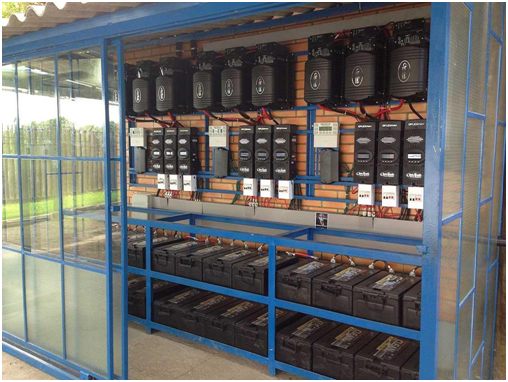
\includegraphics[scale=0.6]{editaveis/figuras/banco_bateria}
\caption[Banco baterias]{Banco de baterias MC 220 Ah na LACTEC em Curitiba\footnotemark}
\label{banco_bateria}
\end{figure}
\footnotetext{Disponível em: https://www.energiapura.com/content/bateria-estacion\%C3\%A1ria-moura-clean-220-ah}
\FloatBarrier

Terminada a fase de alimentação da própria turbina, a energia remanescente na ordem de KW é direcionada por cabeamento subterrâneo até a torre de controle. No meio do caminho, turbina eólica/torre de controle, será instalado um relé com a intenção de controlar a distribuição entre a rede elétrica da região através de um conversor eletrônico e a torre de controle. Em operação normal, a energia será direcionada preferencialmente para a rede elétrica local, evitando desperdícios e visando descontos no consumo energético da torre de controle. No caso de um eventual problema na distribuição energética local, a energia proveniente da turbina será direcionada diretamente para a torre de controle, suprindo suas necessidades de operação e o excedente é direcionada ao carregamento das baterias. A energia na casa de máquinas será utilizada para alimentar computadores, iluminação, tratamento UV e convertida para a alimentação das baterias. 

Para gerarmos energia temos pás, rotor, transmissão por eixo mecânico e gerador elétrico. A partir da energia produzida, os demais componentes da turbina são alimentados eletricamente. Os componentes que recebem alimentação elétrica proveniente do gerador  diretamente na turbina são:
\begin{itemize}
\item Compressor;
\item Sensores;
\item Ventoinha de Ingestão de Ar;
\item Ventoinha de Exaustão de Ar;
\item Sistema de Frenagem.
\end{itemize}

Depois disso, toda a energia remanescente é direcionada para a rede elétrica local/torre de controle. Na central temos os demais componentes que consumirão parte dessa energia. Alguns dos componentes são:
\begin{itemize}
\item Lâmpadas de iluminação;
\item Computadores;
\item Sistema de tratamento;
\item Conversor de Corrente;
\item Baterias.

\end{itemize}

A seguir é apresentado o diagrama esquemático do caminho energético: